\appendix

\Needspace{0.8\textheight}

% \section{Bits-per-Element Sweep}
% \label{app:bpe-sweep}

% \begin{table}[ht!]
% \centering
% \small
% \setlength{\tabcolsep}{6pt}
% \renewcommand{\arraystretch}{1.3}

% % requires: booktabs, array, xcolor, colortbl
% \begin{tabular}{lr|c >{\columncolor{blue!8}}c c c c}
% \toprule
% & & \multicolumn{5}{c}{\textbf{Quantization (bits-per-element)}} \\
% \cmidrule(lr){3-7}
% \textbf{Task} & \textbf{Metric} &
% 4.85 & \textbf{5.03}$^{\dagger}$ & 5.25 & 5.43 & 7.19 \\
% \midrule

% \rowcolor{black!5}
% \multicolumn{7}{l}{\textbf{Coding}} \\
% SciCode & \textit{pass@1 (avg-16), subtask acc} & 43.82 & \textbf{43.88} & 43.45 & 43.27 & 43.44 \\
% \midrule

% \rowcolor{black!5}
% \multicolumn{7}{l}{\textbf{Scientific Reasoning}} \\
% GPQA Diamond & \textit{pass@1 (avg-32), sym.\ correct} & 84.66 & 84.33 & \textbf{84.75} & 84.12 & 84.52 \\
% HLE & \textit{pass@1, judge correct} & 24.24 & 24.84 & 25.00 & 24.98 & \textbf{25.44} \\
% CritPt & \textit{pass@1 (avg-8), accuracy} & 3.04 & 3.93 & \textbf{5.18} & 4.82 & 4.46 \\
% \midrule

% \rowcolor{black!5}
% \multicolumn{7}{l}{\textbf{General}} \\
% AA-Omniscience & \textit{pass@1 (avg-20), judge correct} & 29.21 & \textbf{29.75} & 29.18 & 29.29 & 29.00 \\
%           & \textit{pass@1 (avg-20), non-hallucination} & \textbf{54.13} & 51.59 & 51.84 & 51.70 & 52.81 \\
% IFBench & \textit{pass@1 (avg-8), avg.\ score} & 79.34 & 79.26 & \textbf{79.83} & 79.53 & \textbf{79.83} \\
% \midrule

% \rowcolor{black!5}
% \multicolumn{7}{l}{\textbf{Long Context}} \\
% AA-LCR & \textit{pass@1 (avg-16), judge correct} & 62.25 & \textbf{64.69} & 64.19 & 64.94 & \textbf{65.00} \\
% \bottomrule
% \end{tabular}
% \caption[Bits-per-element sweep]{
%   Bits-per-element (BPE) sweep on a fixed intermediate checkpoint, evaluated with the
%   Nemo Evaluator SDK served on vLLM~v0.20.0. Columns are quantization configurations
%   at increasing effective BPE; the specific recipes are described in
%   Section~\ref{sec:bpe-sweep}. Rows
%   are averaged pass@1 scores, and the best result per row is in bold. The shaded
%   \textbf{5.03} column ($^{\dagger}$NVFP4 with mixed-FP8) is the selected operating
%   point: it is the smallest budget that recovers long-context (AA-LCR) performance,
%   while no benchmark improves beyond run-to-run noise at higher BPE.
% }
% \label{tab:bpe-sweep}
% \end{table}



% \section{SFT}
% \label{appendix:sft}

% \section{RLVR}
% \label{appendix:rlvr}

% \subsection{Jailbreak Robustness Improvements}
% \label{appendix:rlvr_jailbreak_robustness}
% To enable robustness to jailbreaks, a key limitation that we observed in \supermodel was that it was unlearning some of the behavioral cues taught to the model at the SFT stage. This happened because the first attempt at a jailbreak environment used to contain only two verifiers. One binary classification to detect whether the model got jailbroken or not, and if not, a response quality verifier to check whether the refusal response was of "good quality". The definition of "good quality" was simply whether the model provided a templated "I am sorry, I cannot help with that."? or did it actually provide a thoughtful, conversational refusal that fits with the context of the conversation, provides an explanation on why it cannot engage, and optionally redirects the user to a safer topic. 

% Our qualitative observations with \supermodel revealed that this one-size-fits all definition of jailbreak refusal quality assessment is insufficient for good reinforcement learning. This exacerbates the general problem of increased verbosity as RL training progresses, likely because the model reward-hacks into providing longer explanations and redirections to at least satisfy the "refusal with explanations" response quality judge. 

% In reality, while explanations and redirections are good when the user intent is benign and the safety risk is medium to low, it is not the right approach when the user intent is inherently malicious and the safety risk is high (extreme categories like criminal planning, explicitly malicious probing, where the malicious user is trying to find a way to break then model's safety training). In such cases of extreme harm, it is better to block the request conclusively and concisely. There are other categories like suicide and self-harm where the model response must provide appropriate text or call helpline numbers for the user, or cases where the model's ideal response is engagement with a disclaimer rather than a refusal with an explanation. 

% Considering these, it is not enough for the RL reward design to just encourage resisting jailbreaks - how the model resists those jailbreaks and using what behavioral patterns in its response is also paramount. Therefore, in \ourmodel we build prompt metadata to map prompts to response policies and build a suite of nuanced response quality verifiers for each response policy. At training time, the rollouts for each prompt are dynamically routed to the subset of verifiers that are appropriate for the response policy tagged against that prompt. Based on internal qualitative and quantitative evaluations, we see a marked improvement in the quality of responses and an improved understanding of safety and behavioral policies that are applicable in a certain user request, regardless of which jailbreak technique that user request is embedded inside. 

\clearpage
\section{Post-training Evaluations}
\label{appendix:eval}
\subsection{Benchmark Details}
We provide details on specific benchmark settings as below.
\begin{itemize}
    \item \textbf{TauBench V3.} To mitigate premature termination from the user model, we added an additional prompt\footnote{\url{https://github.com/AGI-Eval-Official/tau2-bench-revised}} to the user simulation across all domains. For the banking domain, we used the (terminal\_use) setting which allows the agent to search through the knowledge base through a terminal tool. DeepSeek-V4 models were evaluated under max reasoning. User simulator: GPT-5.2 (low reasoning effort). 8 trial average.
    
    \item \textbf{ProfBench (Search)} We use ProfBench \citep{wang2026profbench} to evaluate model's deep research capability in Professional Work - specifically across Finance MBA, Consulting MBA, Scientific Research in Chemistry PhD and Physics PhD. ProfBench tasks are based on real-world workflows and judged with rubric criteria annotated by professionals working in these domains. Specifically, we run evaluations with a search tool and browse tool enabled in order for the model to identify relevant context from the internet. We run all evaluations at 256K context length without any context management, and report scores averaged over 16 times. 
    
    \item \textbf{Browsecomp}. We evaluate BrowseComp with a custom agentic search harness using Tavily as the search and browsing provider, together with terminal access. To avoid loading all retrieved web content into the model context, search and browse results are persisted to a per-task disk workspace; the model receives only metadata/snippets and can selectively inspect saved pages with shell commands such as grep, head, and sed. This allows the model to retrieve relevant evidence surgically, slows context growth, and preserves all previously collected search information across context resets.
   
    \item \textbf{Vals.ai Finance Agent Benchmark (FAB v1.1).} We evaluate on the Vals.ai Finance Agent Benchmark \citep{bigeard2025finance}, which tests agents on entry-level financial analyst tasks spanning nine different categories, from simple retrieval to financial modeling and market analysis. While the full benchmark reports on a private test set of 337 questions, we evaluate on 200 questions: the 50 publicly available validation samples augmented with 150 additional samples from the privately licensed validation set. Agents are provided four tools in the no-web-search condition: EDGAR search (via SEC API), an HTML page parser, a retrieval tool for querying previously extracted content, and a \texttt{submit} tool for producing the final answer. In the web search condition, a fifth tool, Google web search via Tavily, is additionally available. Since the benchmark is grounded in SEC filings, most questions are expected to be answerable from EDGAR directly; web search serves as a supplementary signal. Accuracy is judged against expert-written ground-truth answers using an LLM-as-judge (GPT-5.2, mode of three evaluations). We closely follow the open-source evaluation harness.\footnote{\url{https://github.com/vals-ai/finance-agent}}
    
\end{itemize}


\subsection{Harness Robustness}

\begin{figure*}[ht]
    \centering

    \begin{subfigure}[t]{0.48\linewidth}
        \centering
        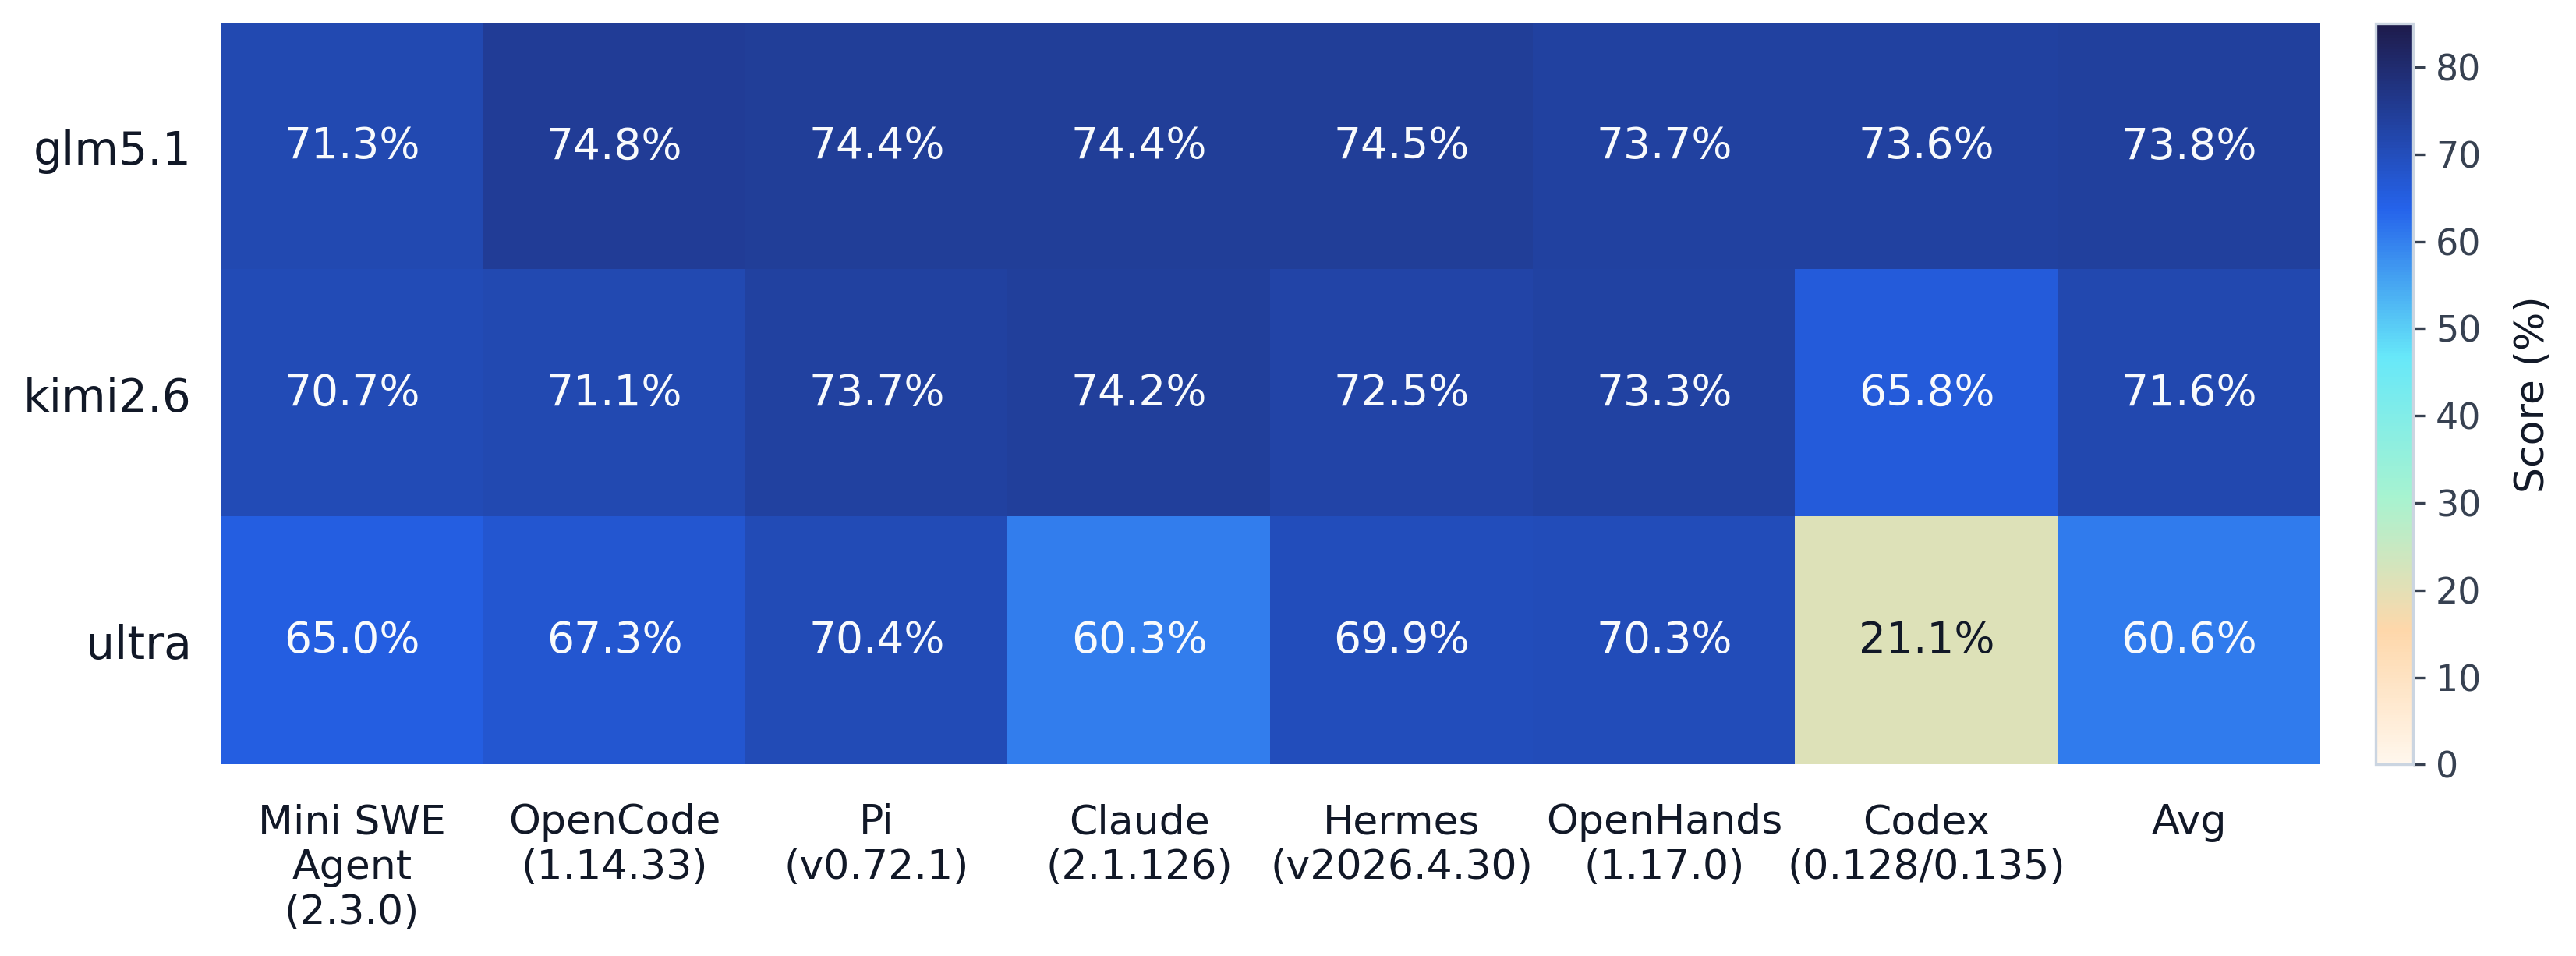
\includegraphics[width=\linewidth]{figures/swebench_verified_agent_matrix.png}
        \caption{SWE-bench Verified}
        \label{fig:swebench_agent_matrix}
    \end{subfigure}
    \hfill
    \begin{subfigure}[t]{0.48\linewidth}
        \centering
        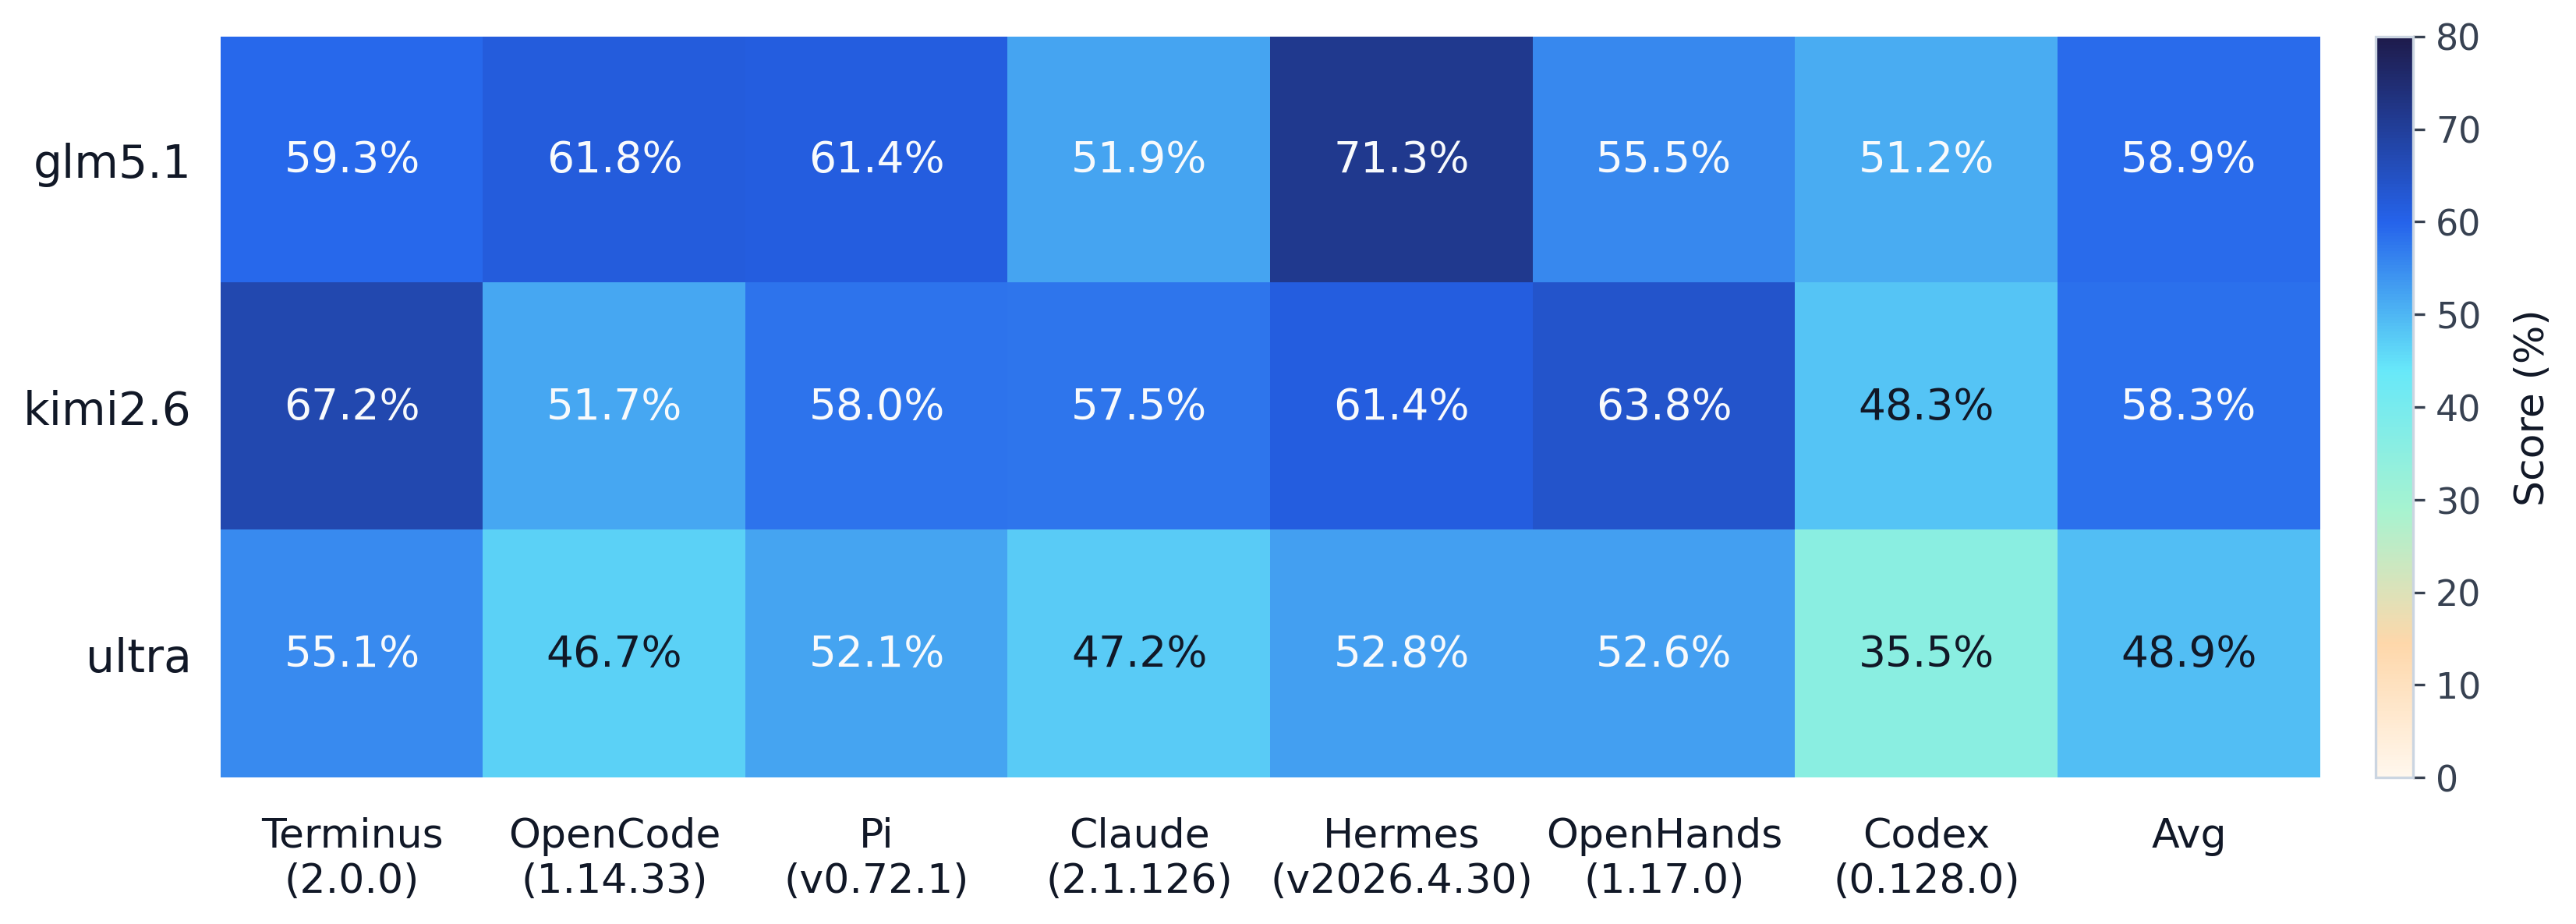
\includegraphics[width=\linewidth]{figures/terminal_bench_2_1_agent_matrix.png}
        \caption{Terminal-Bench 2.1}
        \label{fig:terminal_agent_matrix}
    \end{subfigure}

    \caption{Agent and model matrices for SWE-bench Verified and Terminal-Bench 2.1.}
    \label{fig:agent_model_matrix}
\end{figure*}

Harness Robustness is a key part of the post-training stage for Nemotron-3 Ultra. We categorize all of the task distributions into five verticals, including:
\begin{itemize}
    \item Zero to One Terminal Use and Software Engineering Task
    \item Existing Repo Bug Fixing Tasks
    \item Office and General Productivity Tasks
    \item General/Multi-domain Knowledge Tasks
    \item Search Tasks
\end{itemize}

For each of these input task distributions, we ensure that the model is trained under at least two of the following harnesses:
\begin{itemize}
    \item Stirrup
    \item OpenHands
    \item OpenCode
    \item Terminus
    \item Droid
    \item Custom Internal Harnesses
\end{itemize}

The prevention of the model being trained under a single harness for any given task distribution allows for better generalization and robustness when the model is used under dynamic execution contexts in real world settings. The performance of \ourmodel on different harnesses are shown in Figure \ref{fig:agent_model_matrix}.

